\documentclass[a4paper,12pt]{article}

\usepackage[height=22.5cm, width=17.5cm]{geometry} 

\usepackage{graphicx}
\graphicspath{ {./images/} }

\usepackage[french]{babel}


\usepackage{hyperref}


\usepackage[T1]{fontenc} % font encoding
\usepackage{lmodern} % font


	
	
	
	
	\begin{document}
		\title{Analyse des résultats du championnat du monde de \\  Backyard Ultra 2023}
		\author{Vincent Gozé}
		\date{20 janvier 2025}
		\maketitle
\begin{center}
	\noindent\rule{13cm}{0.3pt}\\ ~ \\
	\textbf{Format de course: le Backyard Ultra}
\end{center}


Le Backyard Ultra est un format de course inventé par Gary Cantrell, alias Lazarus Lake ou Laz, le célèbre inventeur de la Barkley. Il raconte que durant sa jeunesse, il imaginait une course où il fallait courir environ 4 miles par heures jusqu'à ce qu'il ne reste qu'un coureur. Ce n'est qu'en 2011 que la première course de ce genre a été organisée par Laz, dans son jardin ! Pour arrondir la distance parcourue sur une journée, la distance du tour est d'exactement $4.16667$ miles, soit environ $6.7$ kilomètres, ce qui correspond à 100 miles pour 24 heures.  Laz décrit la difficulté de ce format de la manière suivante: \og	The hardest part of the course is between your chair and the starting corral.\fg{}

\medskip

\begin{figure}[b]
	
	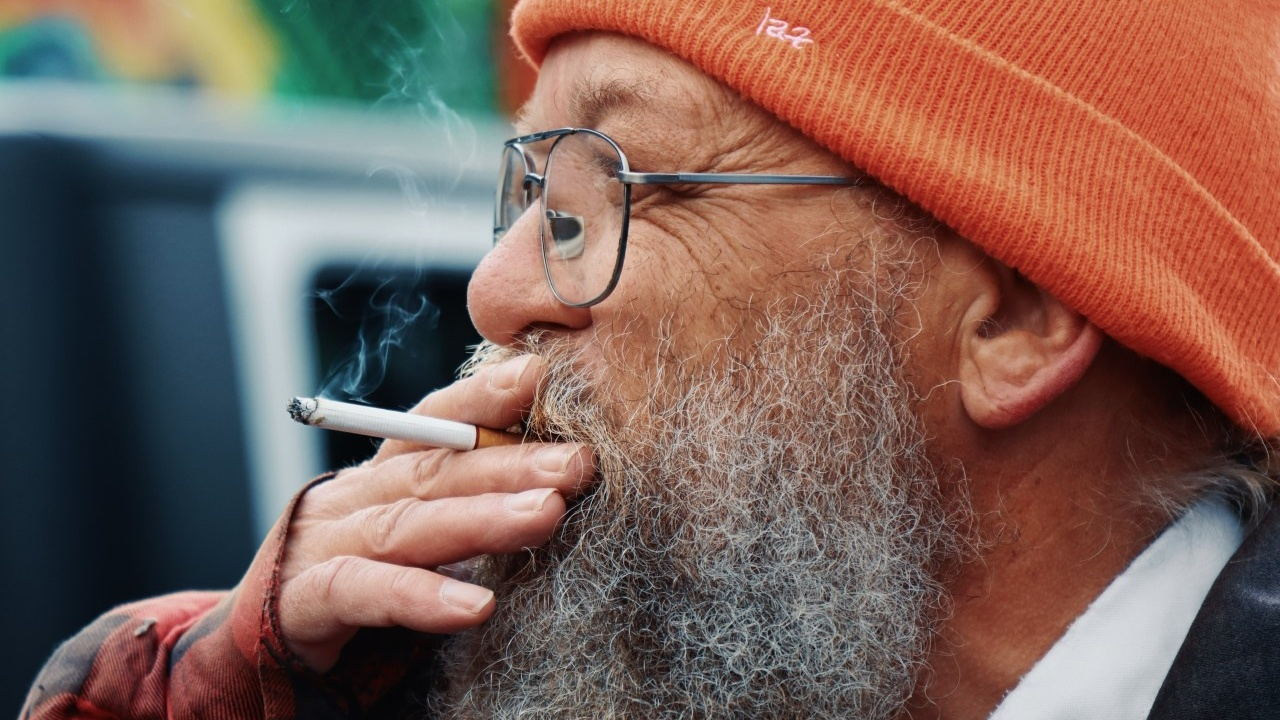
\includegraphics[scale=0.15]{Laz}
	\centering
	\caption{L'emblématique Lazarus Lake}
\end{figure}

Concrètement, toutes les heures, le départ d'une boucle est lancé et les coureurs doivent réaliser le tour de $6.7$ kilomètres en moins de $60$ minutes. S'ils arrivent avant la fin du temps imparti, ils peuvent profiter du temps restant pour s'alimenter, se changer ou se reposer dans leur tente et être assistés par leur entourage. 
Il y a trois façons d'être éliminé:
\begin{itemize}
	\item[$\bullet$] OVER pour Over Time on Loop: le coureur termine la boucle au-delà du temps imparti;
	\item[$\bullet$] RTC pour Refuse to Continue: le coureur choisit de ne pas prendre le départ du prochain tour;
	\item[$\bullet$] DNC pour Did Not Complete Loop: le coureur prend le départ du tour mais ne le complète pas entièrement (en faisant demi-tour par exemple).
\end{itemize}




\medskip
La course continue jusqu'à ce qu'il ne reste plus qu'un concurrent. Le vainqueur est déclaré si il parvient à effectuer un tour supplémentaire après l'élimination de tous les autres concurrents. Il y a donc, au maximum, un seul finisher. Pourquoi au maximum ? Parce que si les deux derniers concurrents sont éliminés en même temps, il n'y a pas de vainqueur !

\medskip

Durant la première édition, le vainqueur a réalisé 18 tours. Ce record a été amélioré de nombreuses fois et a été porté à 110 boucles lors du championnat du monde par équipes 2024. 

\begin{center}
	\textbf{Le championnat du monde 2023}
\end{center}

Le championnat du monde 2023 a eu lieu à Bell Buckle dans le Tennessee, toujours autour de la propriété de Laz. La course a démarré à 7 heures du matin et la particularité était la distinction entre le circuit réalisé de jour, sur chemin et en forêt et présentant $154$m de dénivelé positif, et le circuit de nuit, exclusivement sur route et avec $40$m de dénivelé positif. Il faut donc adapter sa stratégie selon le type de circuit. Les règles sont simples: \og Trail Loop 11 Hours, then Road Loop 13 Hours - Repeat as Necessary.\fg{}. Les conditions météorologiques sont clémentes avec un temps sec, une température autour de 25°C le jour et 10°C la nuit.


%\begin{figure}[h]
%	
%	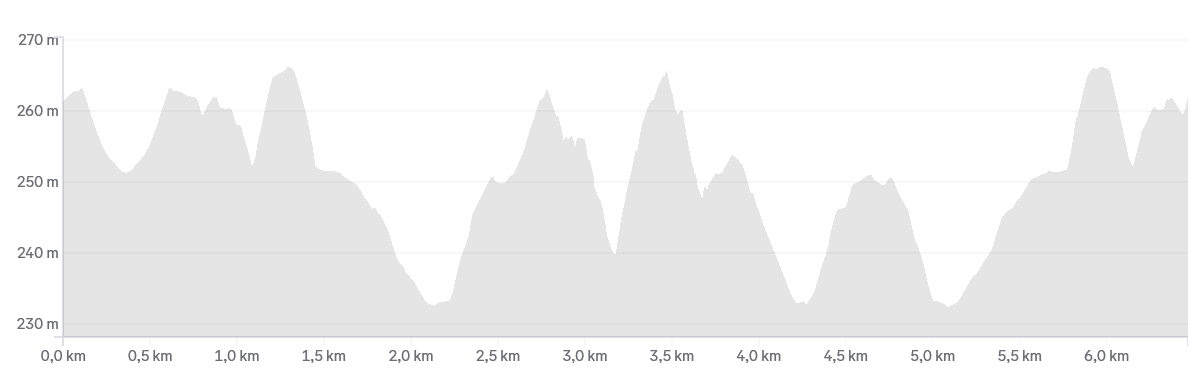
\includegraphics[scale=0.4]{Strava}
%	\centering
%	\caption{Le parcours de jour, qui présente un dénivelé plus important}
%\end{figure}

\medskip
Il y avait $75$ coureurs au départ. Après $24$ heures, $72$ coureurs étaient encore en course. Au bout de $48$ heures, il y en avait encore $47$ et après $72$ heures, $23$ coureurs étaient encore en course. La victoire s'est jouée à l'entame de la cinquième nuit: après la 107ème boucle, la dernière du cinquième jour sur la partie chemin, deux coureurs sont encore en course: Harvey Lewis et Ihor Verys. À l'entame de la nuit, Verys décide de ne pas repartir pour une 108ème boucle. Il suffit donc à Lewis de boucler encore un tour sur le circuit route pour empocher la victoire. Il réalise cette boucle en 47m31s, après plus de quatre jours et demi de course.

\begin{figure}[!h]
	
	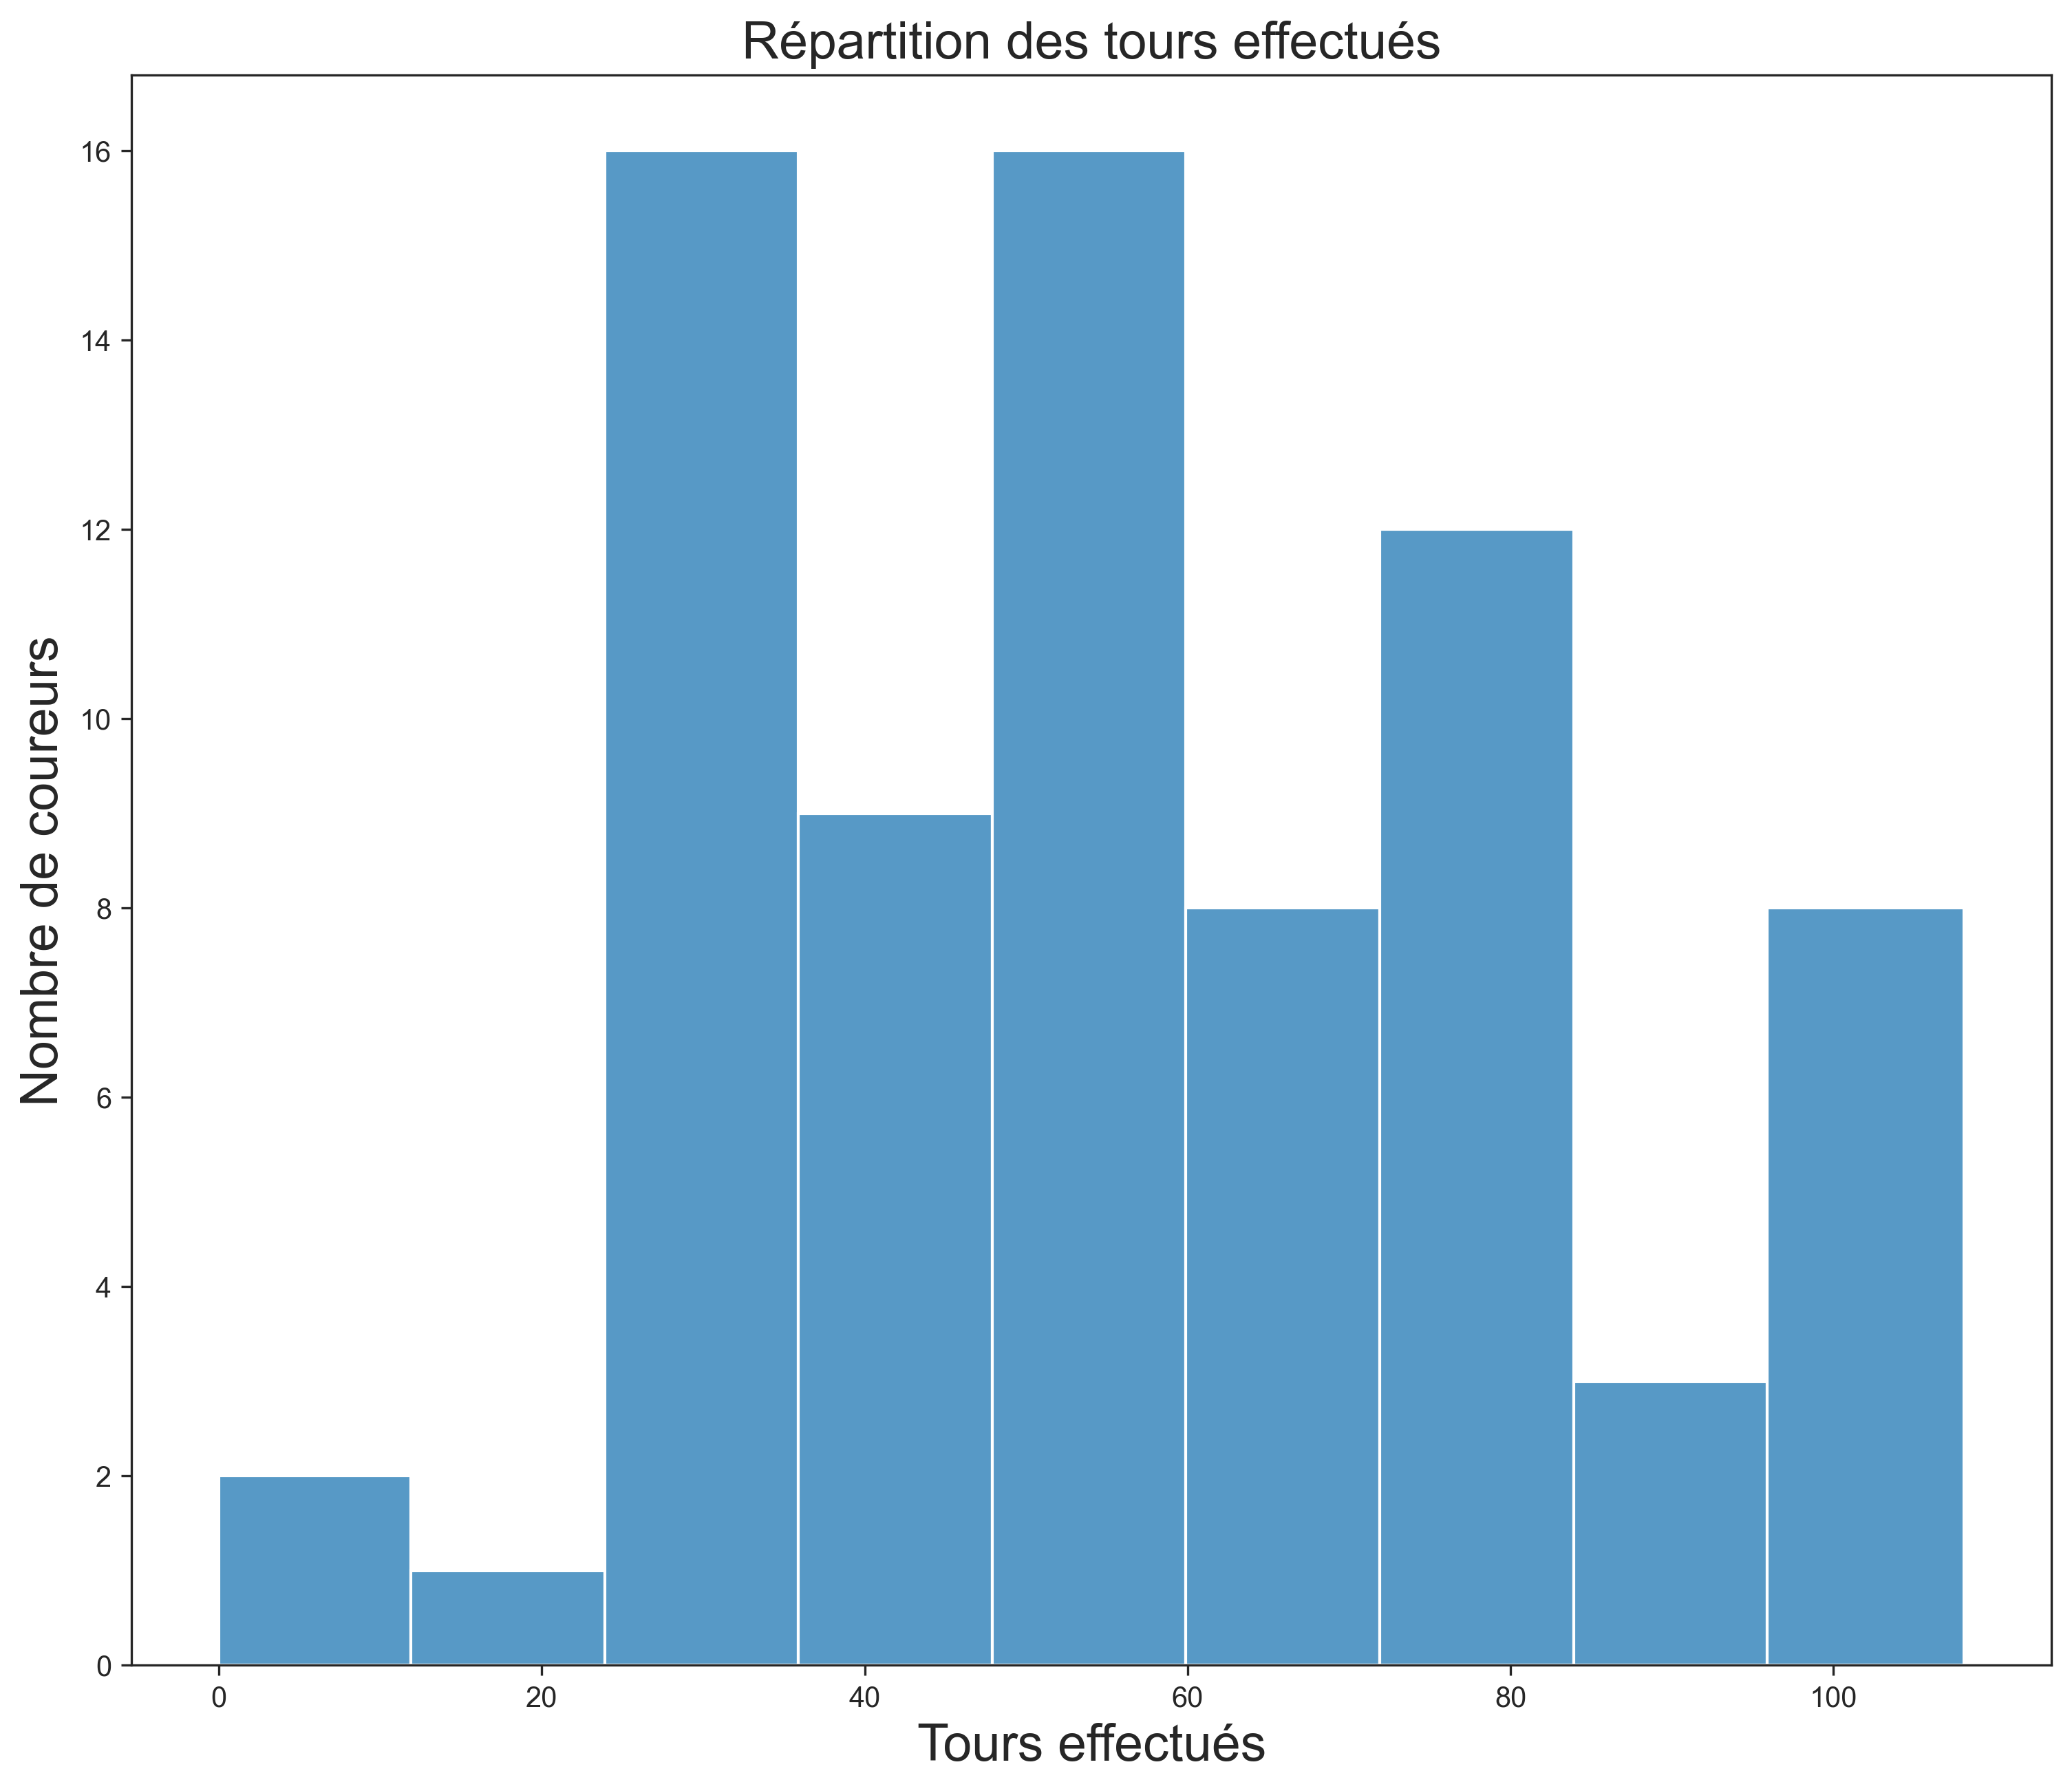
\includegraphics[scale=0.3]{histogram}
	\centering
	\caption{Répartition des tours effectués}
\end{figure}
\medskip
Dans la suite, nous essayons de déterminer la stratégie à adopter: faut-il être lent et maintenir un rythme modéré pour préserver son énergie ou au contraire être plus rapide pour maximiser les moments de repos ? Pour cela, on peut commencer par analyser les temps au tours des deux premiers coureurs.

\begin{figure}[!h]
	\centering
		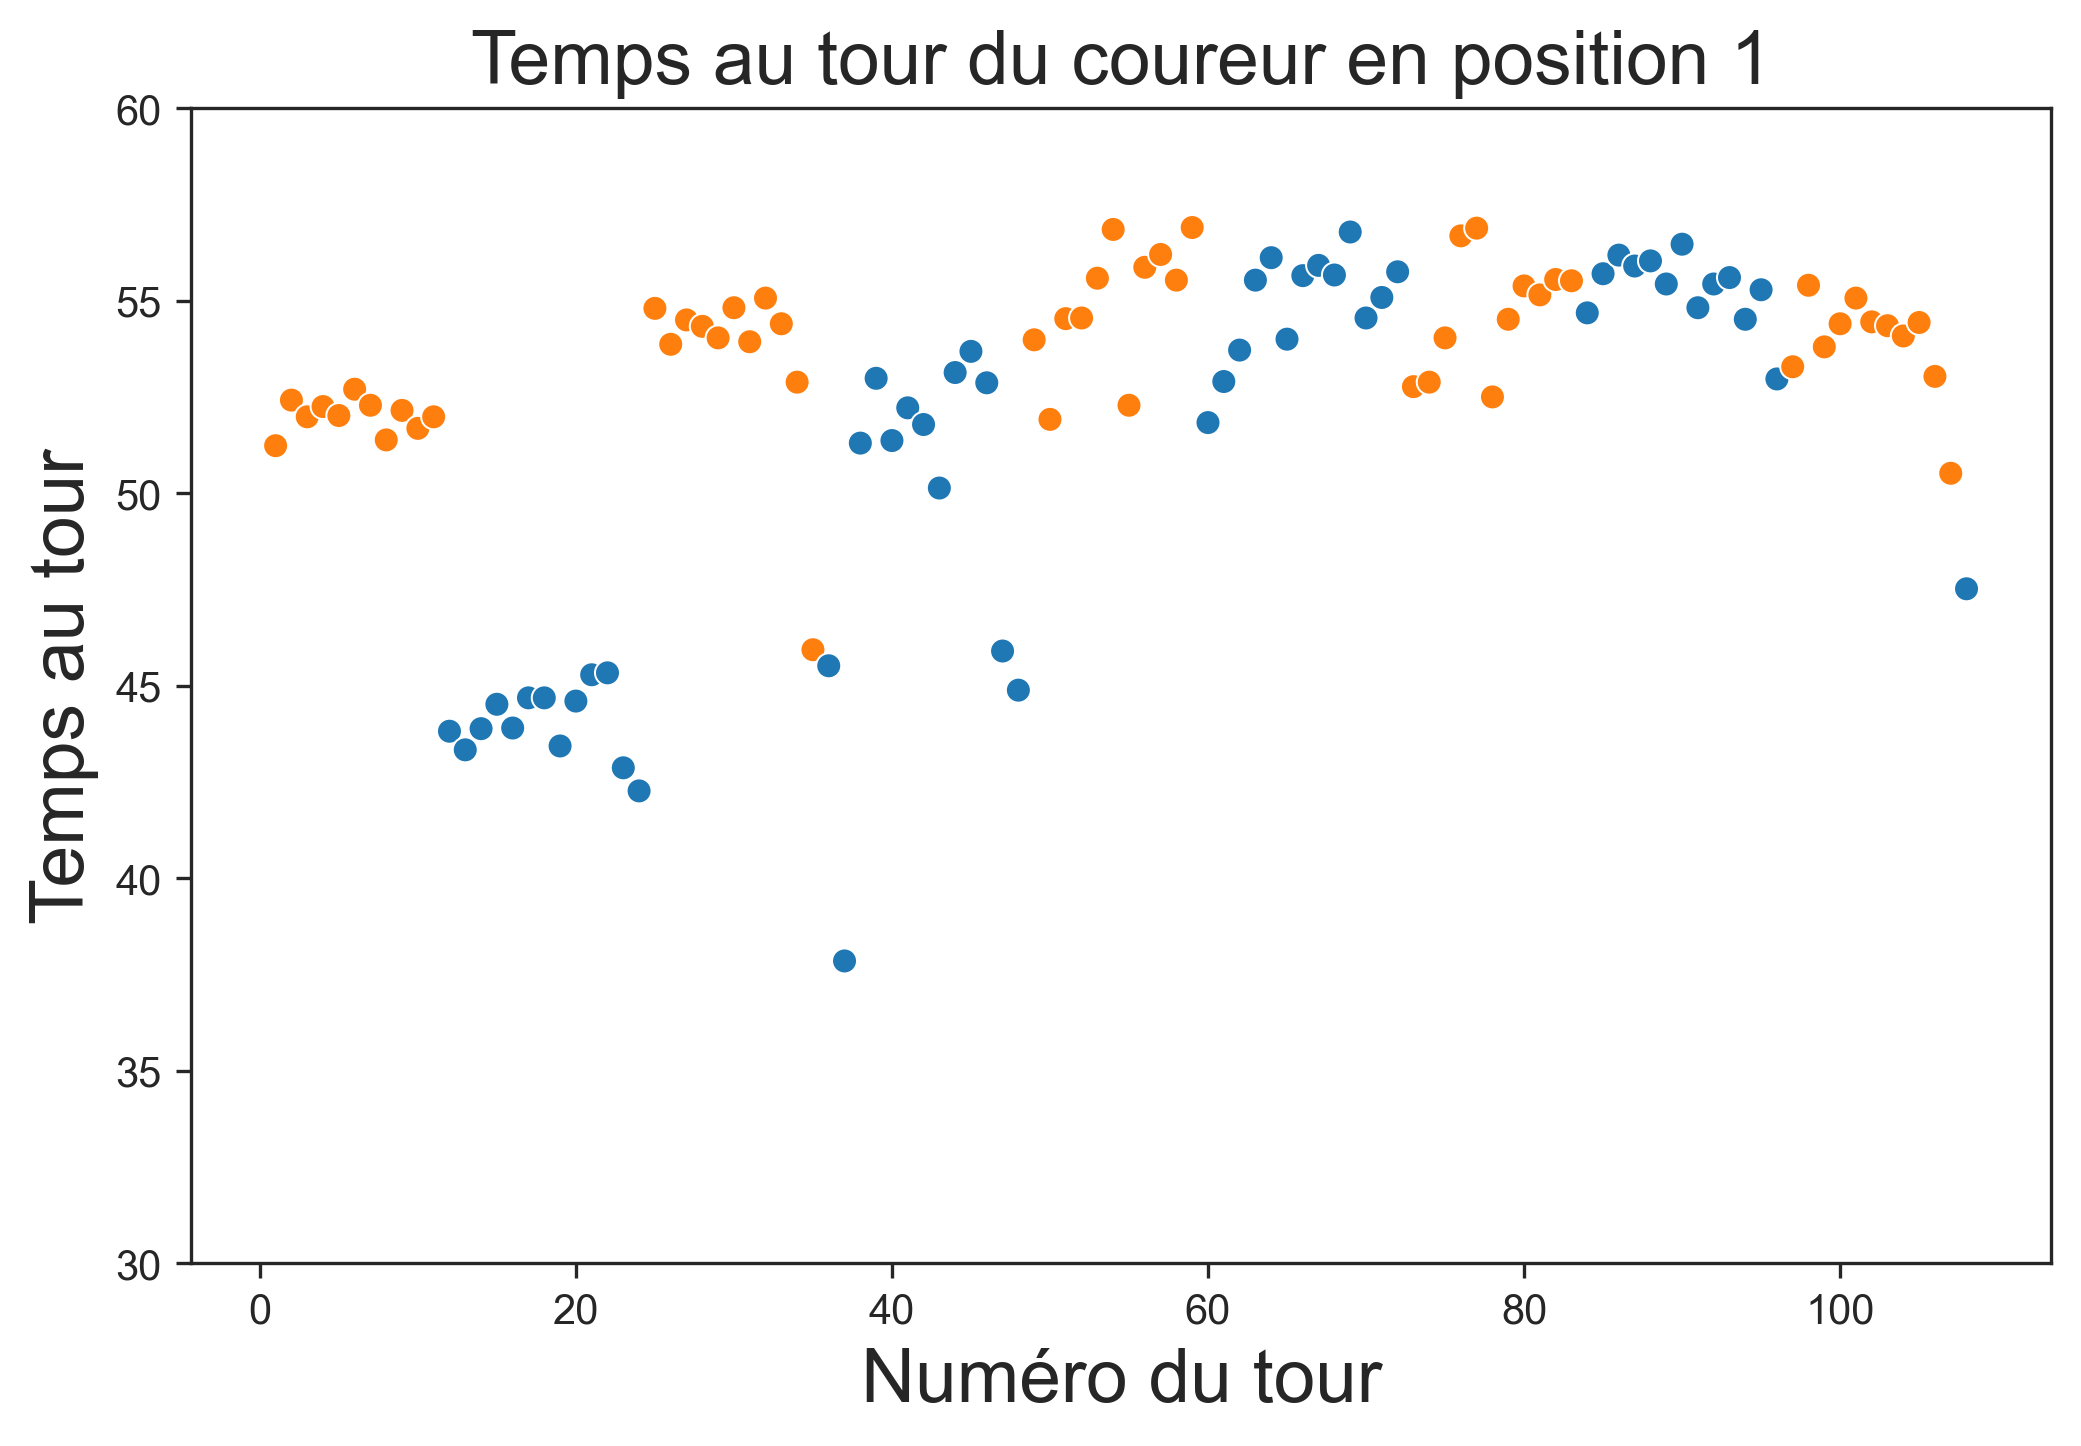
\includegraphics[scale=0.45]{tempstour1}
		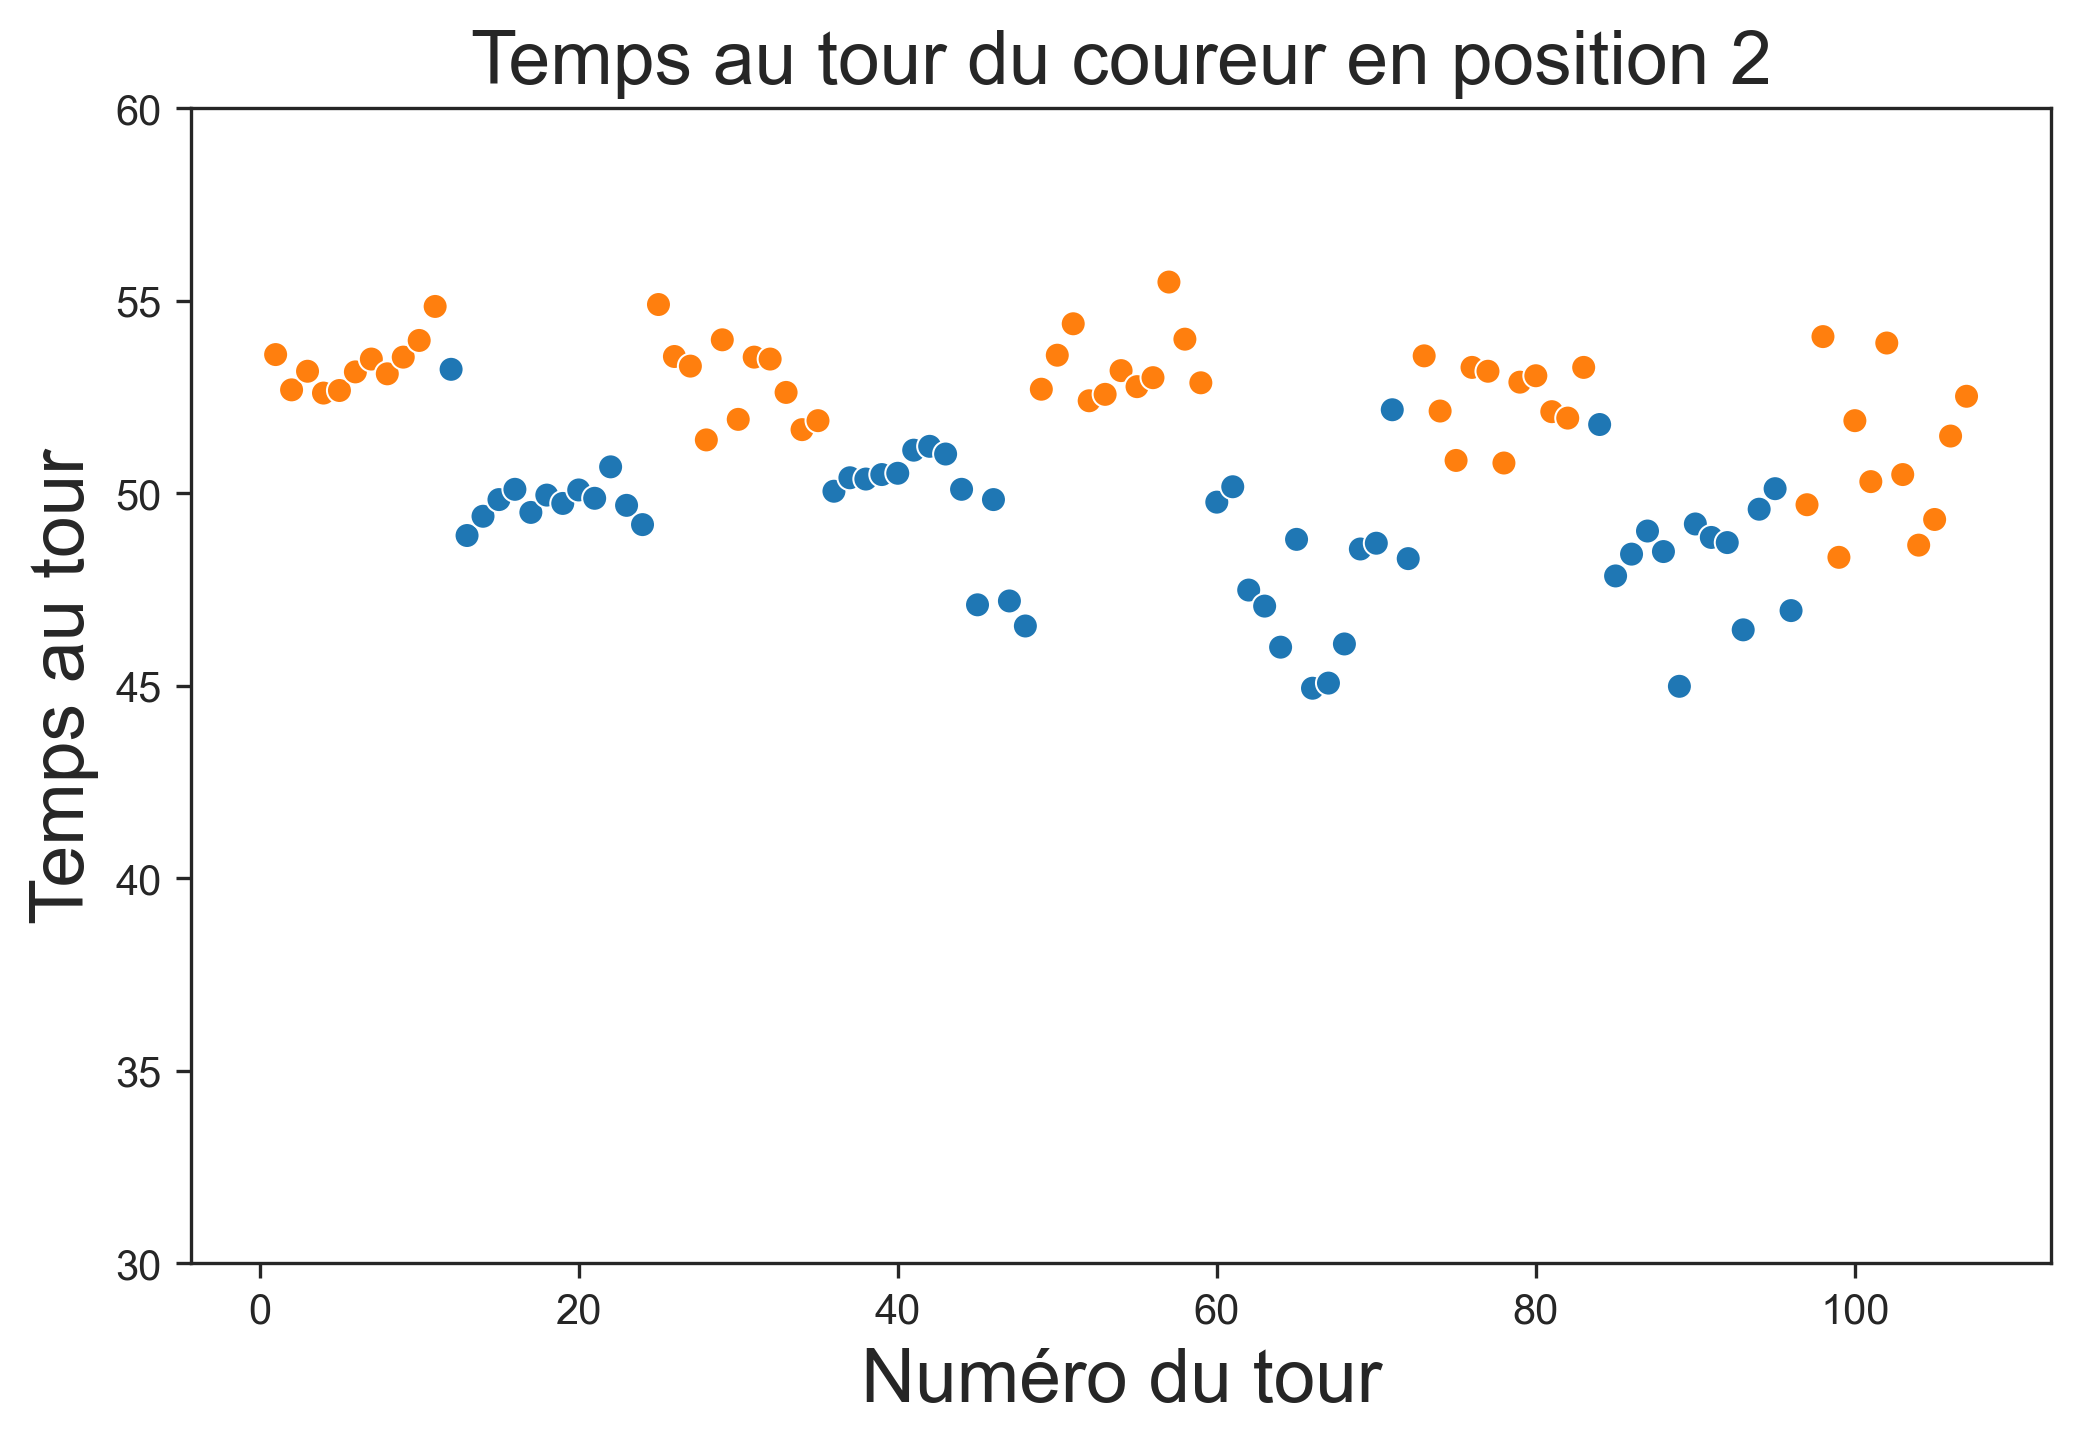
\includegraphics[scale=0.45]{tempstour2}
		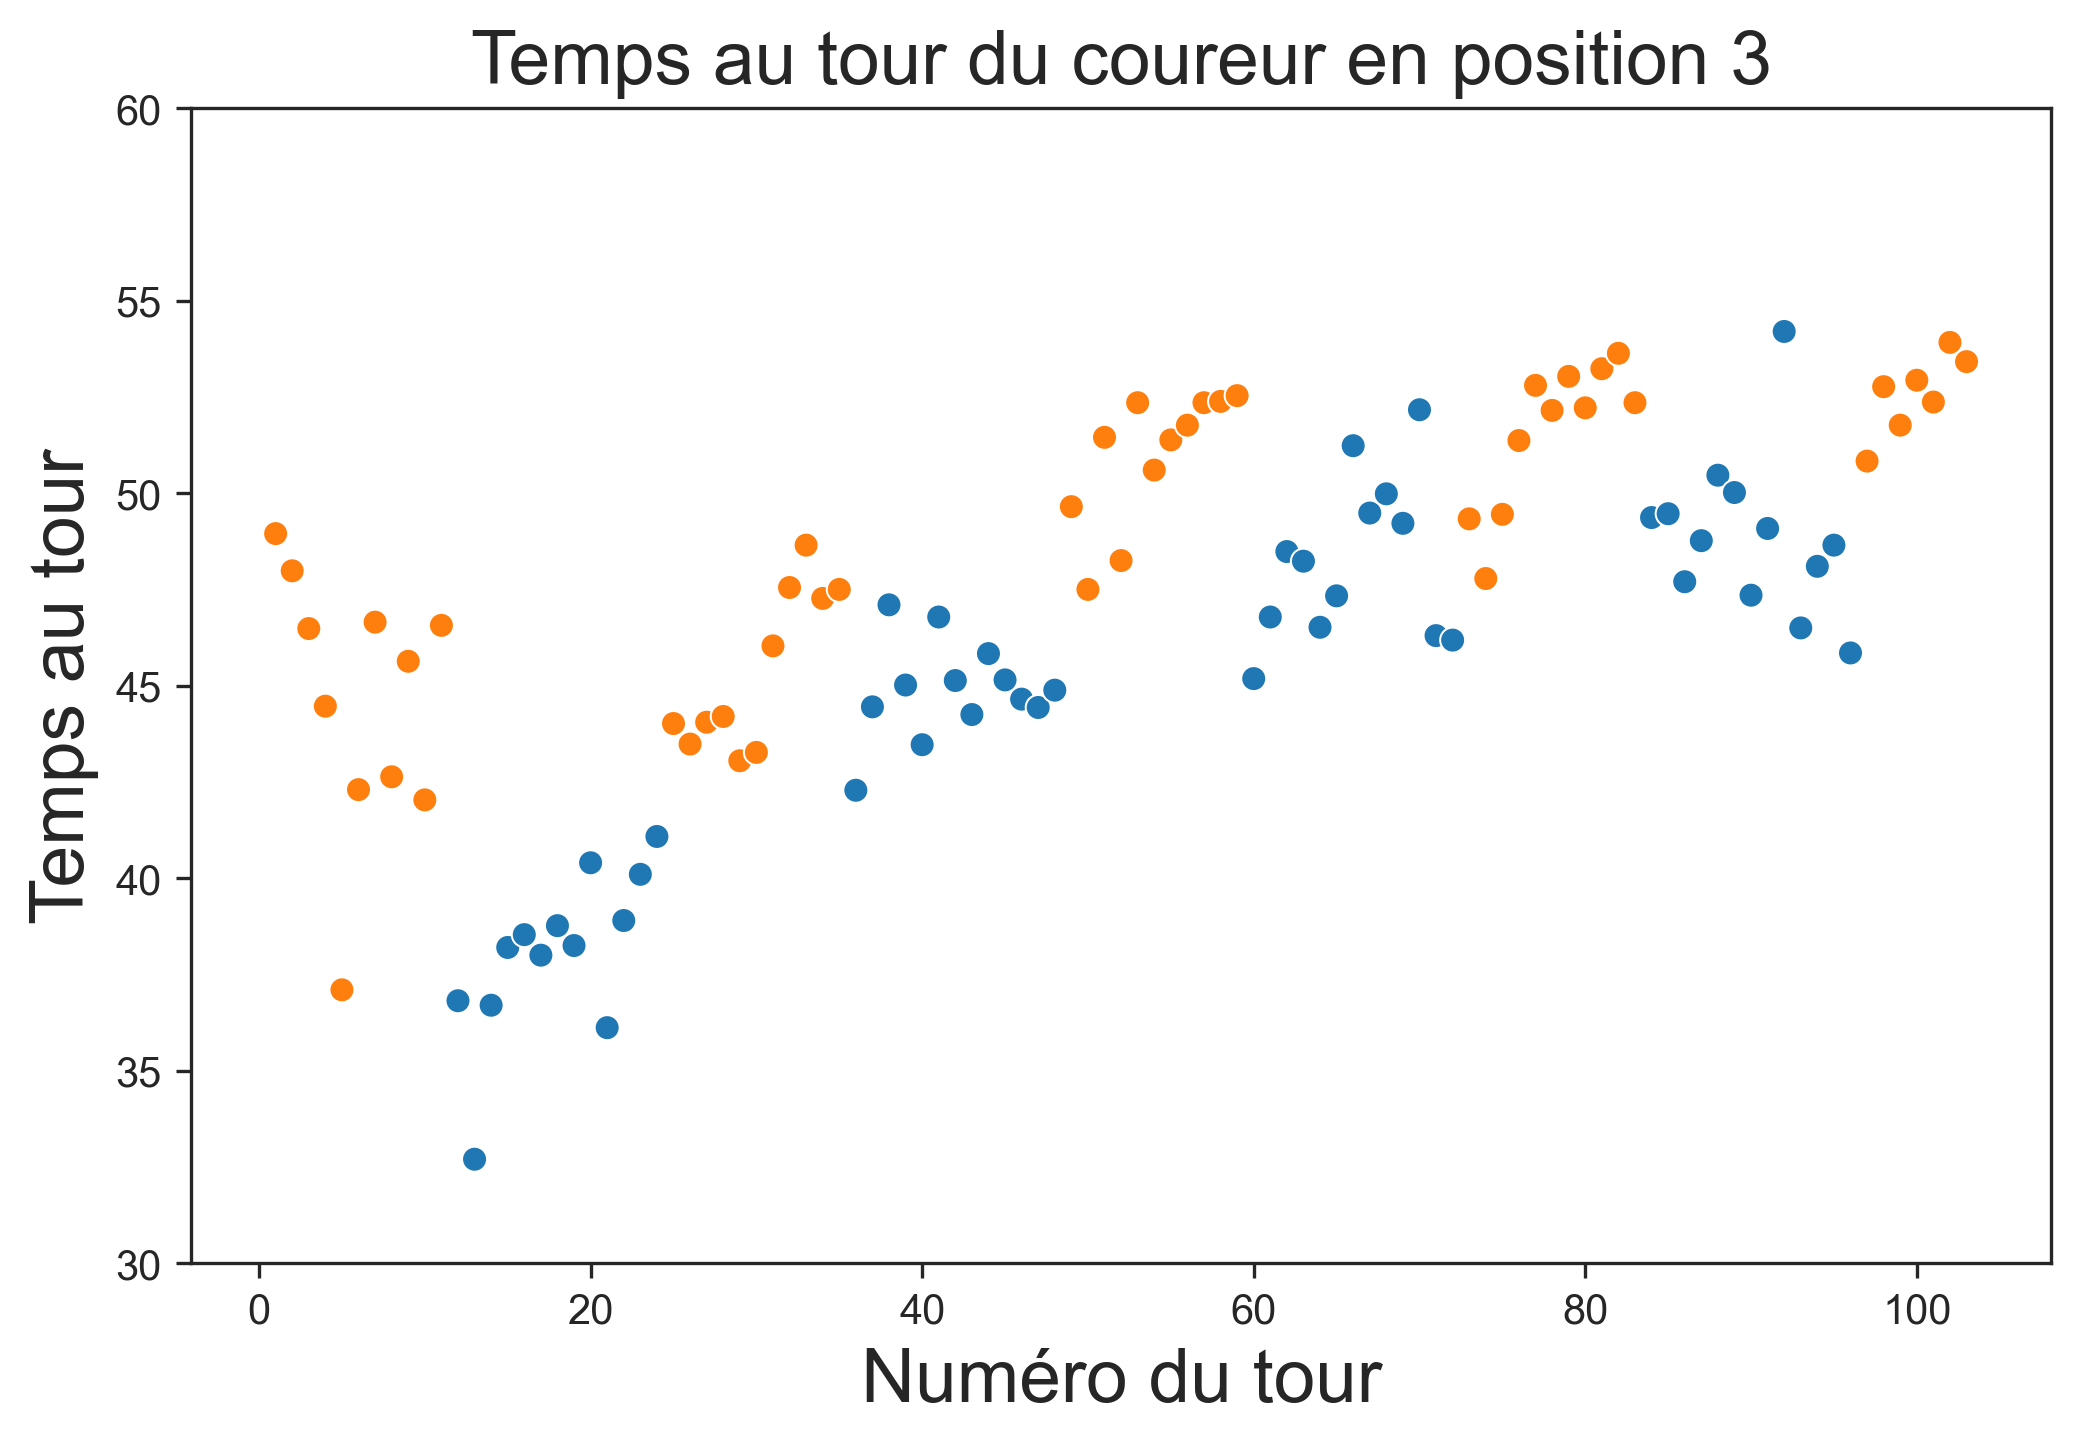
\includegraphics[scale=0.45]{tempstour3}
		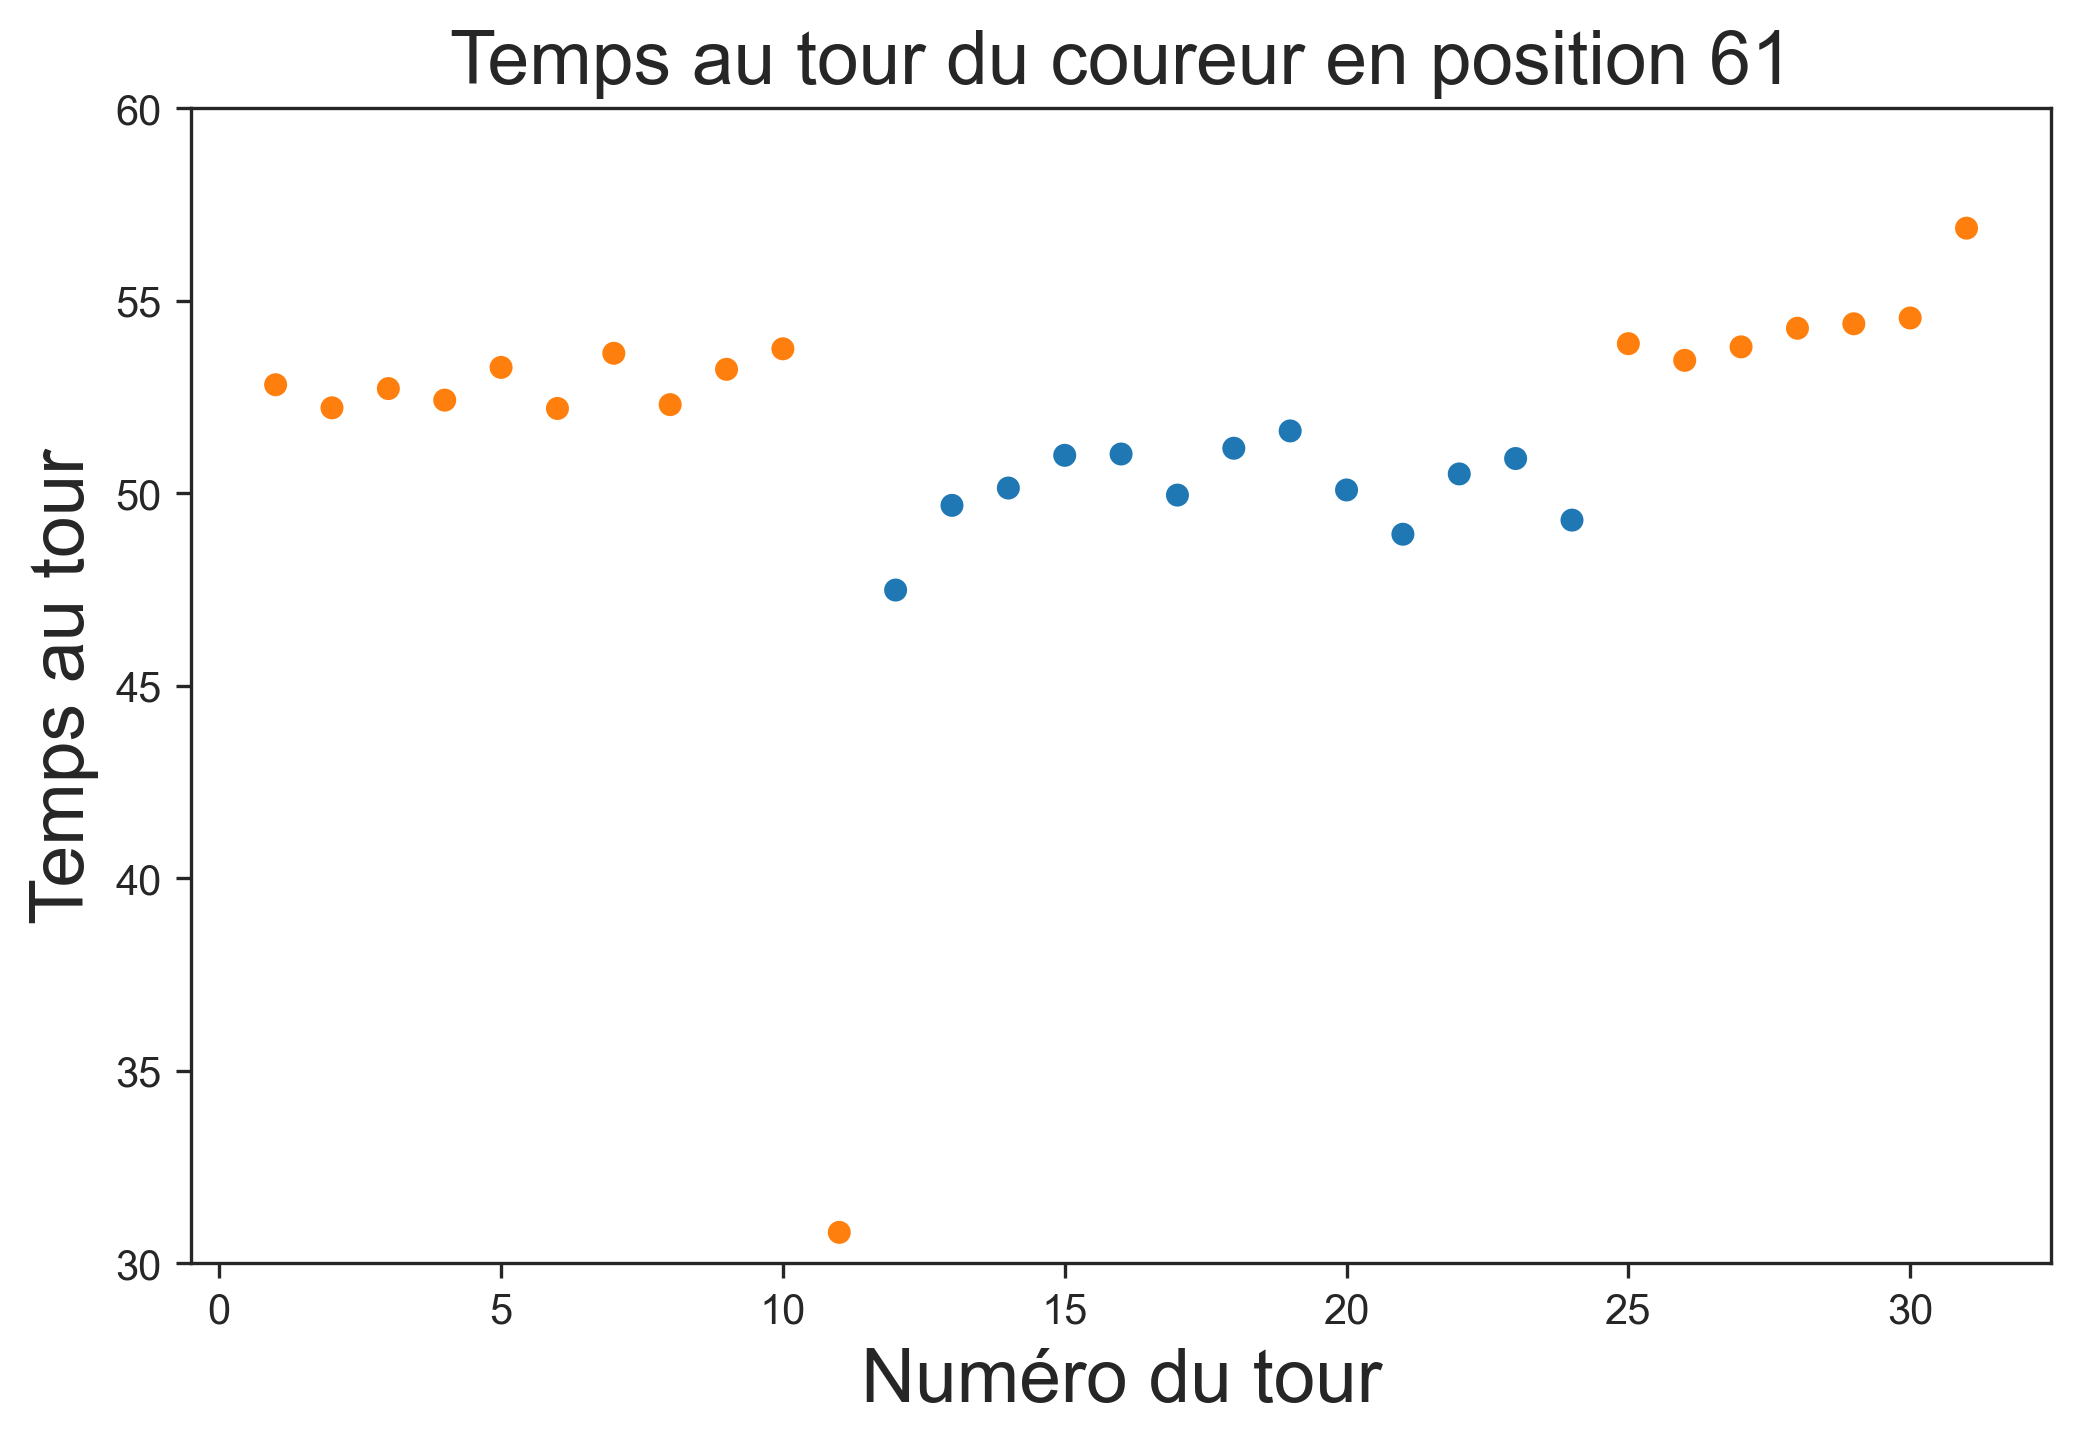
\includegraphics[scale=0.45]{tempstour61}
	\caption{Temps au tour de certains coureurs}
\end{figure}

\medskip
On remarque que les stratégies sont différentes d'un coureur à l'autre. Les deux premiers, Lewis et Verys, ont été assez réguliers tout au long de la course bien qu'adoptant des allures différentes. Bartosz Fudali, arrivé en troisième position, était beaucoup plus irrégulier. Il a même établi le record sur le tour de nuit en 32m42s sur la 13ème boucle. Quant à Visa Kivinen, 61ème de la course, il a adopté une stratégie assez étrange, avec des temps plutôt réguliers sauf pour la 11ème boucle, la dernière du premier jour, avec le record absolu de 30m48s, et ça sur le circuit avec le plus de dénivelé.
\begin{center}
	\textbf{Analyse des moyennes et écarts-types des temps au tour}
\end{center}

Afin d'effectuer l'analyse des stratégies des différents coureurs, nous calculons la moyenne et l'écart-type de leurs temps au tour sur chaque jour ou chaque nuit. Par exemple, \texttt{mean\_day\_1} désigne la moyenne d'un coureur sur le premier jour, c'est à dire les 11 premiers tours, et \texttt{std\_night\_2} désigne l'écart-type de l'échantillon des temps au tour d'un coureur durant la deuxième nuit, c'est à dire les tours 36 à 48.
\medskip

Pour commencer, on se pose la question suivante: Parmi les coureurs ayant effectué 24 tours ou plus, quel variable parmi \texttt{mean\_day\_1}, \texttt{std\_day\_1}, \texttt{mean\_night\_1} et \texttt{std\_night\_1} influence le plus le nombre total de tours effectués ?

\medskip

Pour cela, nous utilisons les Random Forests, un algorithme d'intelligence artificielle basé sur un ensemble d'arbres de décisions. Habituellement utilisé pour effectuer des prédictions, nous l'exploitons ici pour calculer la \textit{feature importance}: une mesure de l'importance d'une variable dans la prise de décision de l'algorithme. Nous calculons également le coefficient de corrélation de Spearman de chaque variable avec le nombre de tours effectués. Nous obtenons ainsi le graphique suivant.
\begin{figure}[!h]
	
	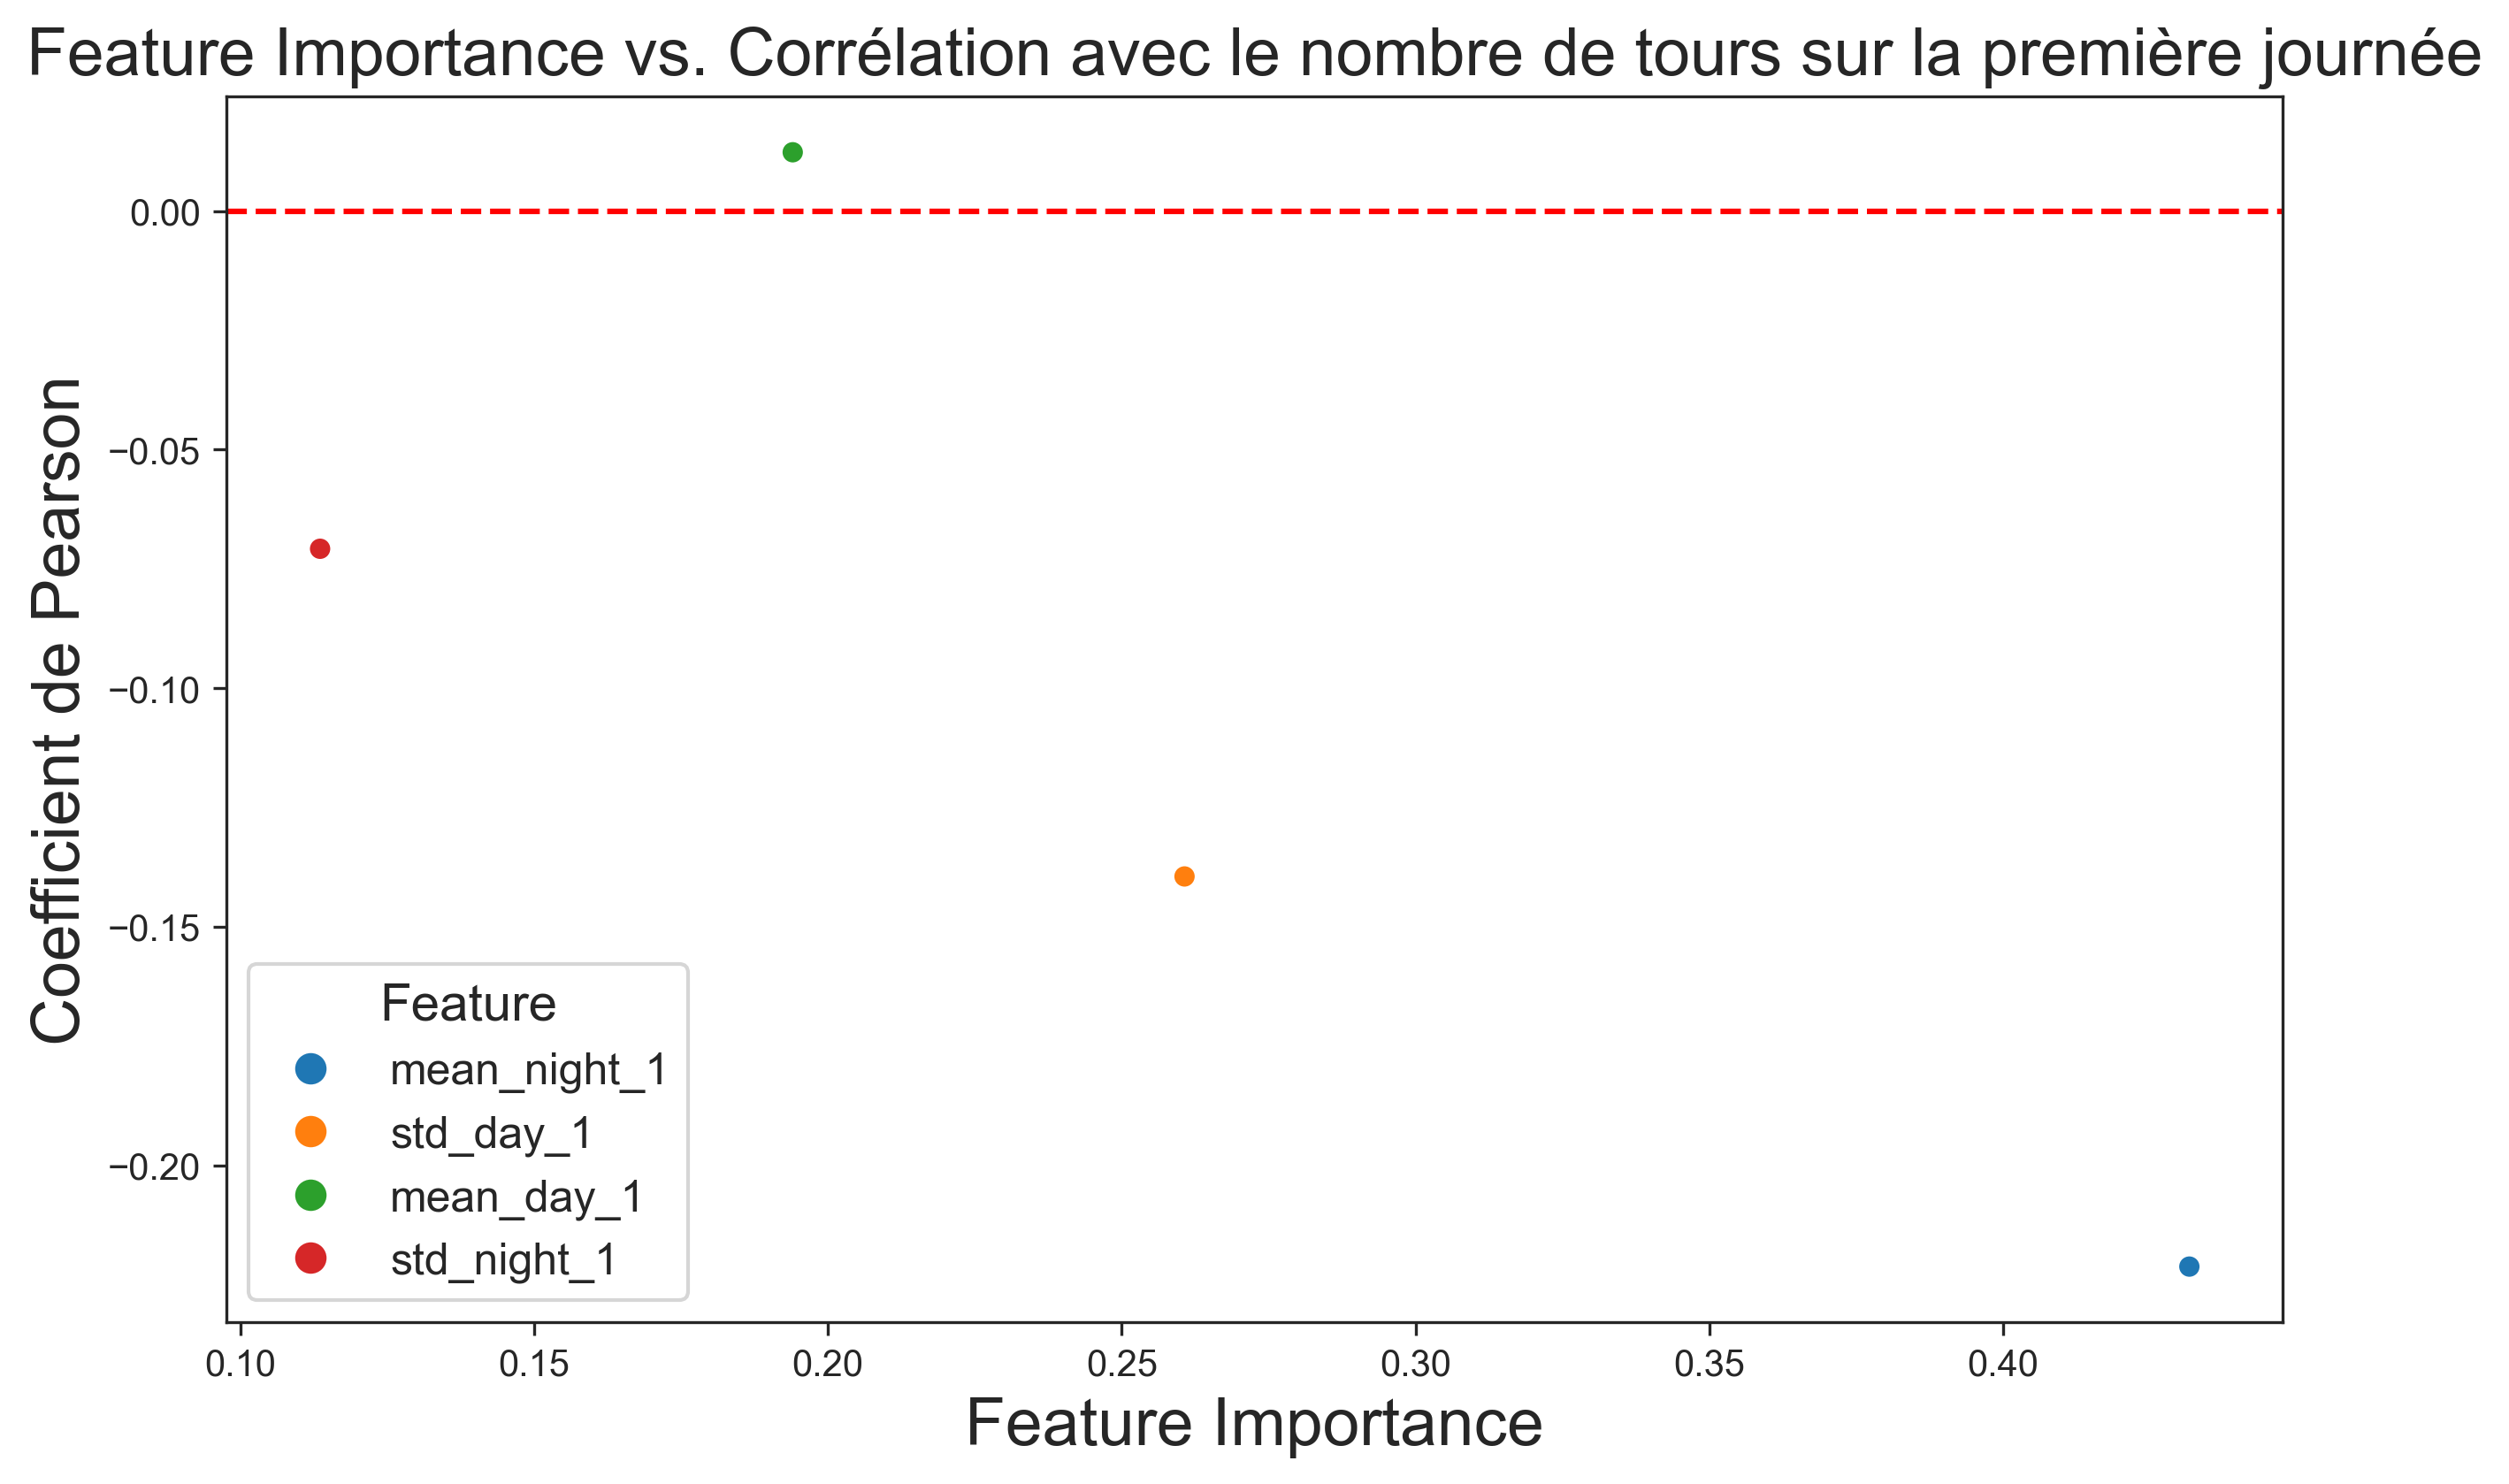
\includegraphics[scale=0.41]{feature1}
	\centering
	\caption{Feature importance et corrélation sur le premier tour}
\end{figure}




La variable la plus importante est \texttt{mean\_night\_1} et le coefficient de corrélation associé est négatif: cela signifie qu'en moyenne, plus la moyenne des temps au tour de la première nuit est basse, plus le nombre de tours est élevé. La deuxième variable la plus importante est \texttt{std\_day\_1} et le coefficient de corrélation est aussi négatif: plus le coureur est régulier durant le premier jour, plus il a de chances d'aller loin. Ainsi, parmi les coureurs ayant réalisé plus de 24 tours, ceux qui vont le plus loin sont ceux qui sont réguliers le premier jour et plus rapide que les autres durant la première nuit, ce dernier point peut s'expliquer par le fait que les coureurs qui vont bientôt abandonner sont probablement déjà en souffrance dans cette première nuit.
\medskip


On réalise maintenant la même analyse en conservant uniquement les coureurs ayant réalisés plus 48 tours ou plus.
\begin{figure}[!h]
	
	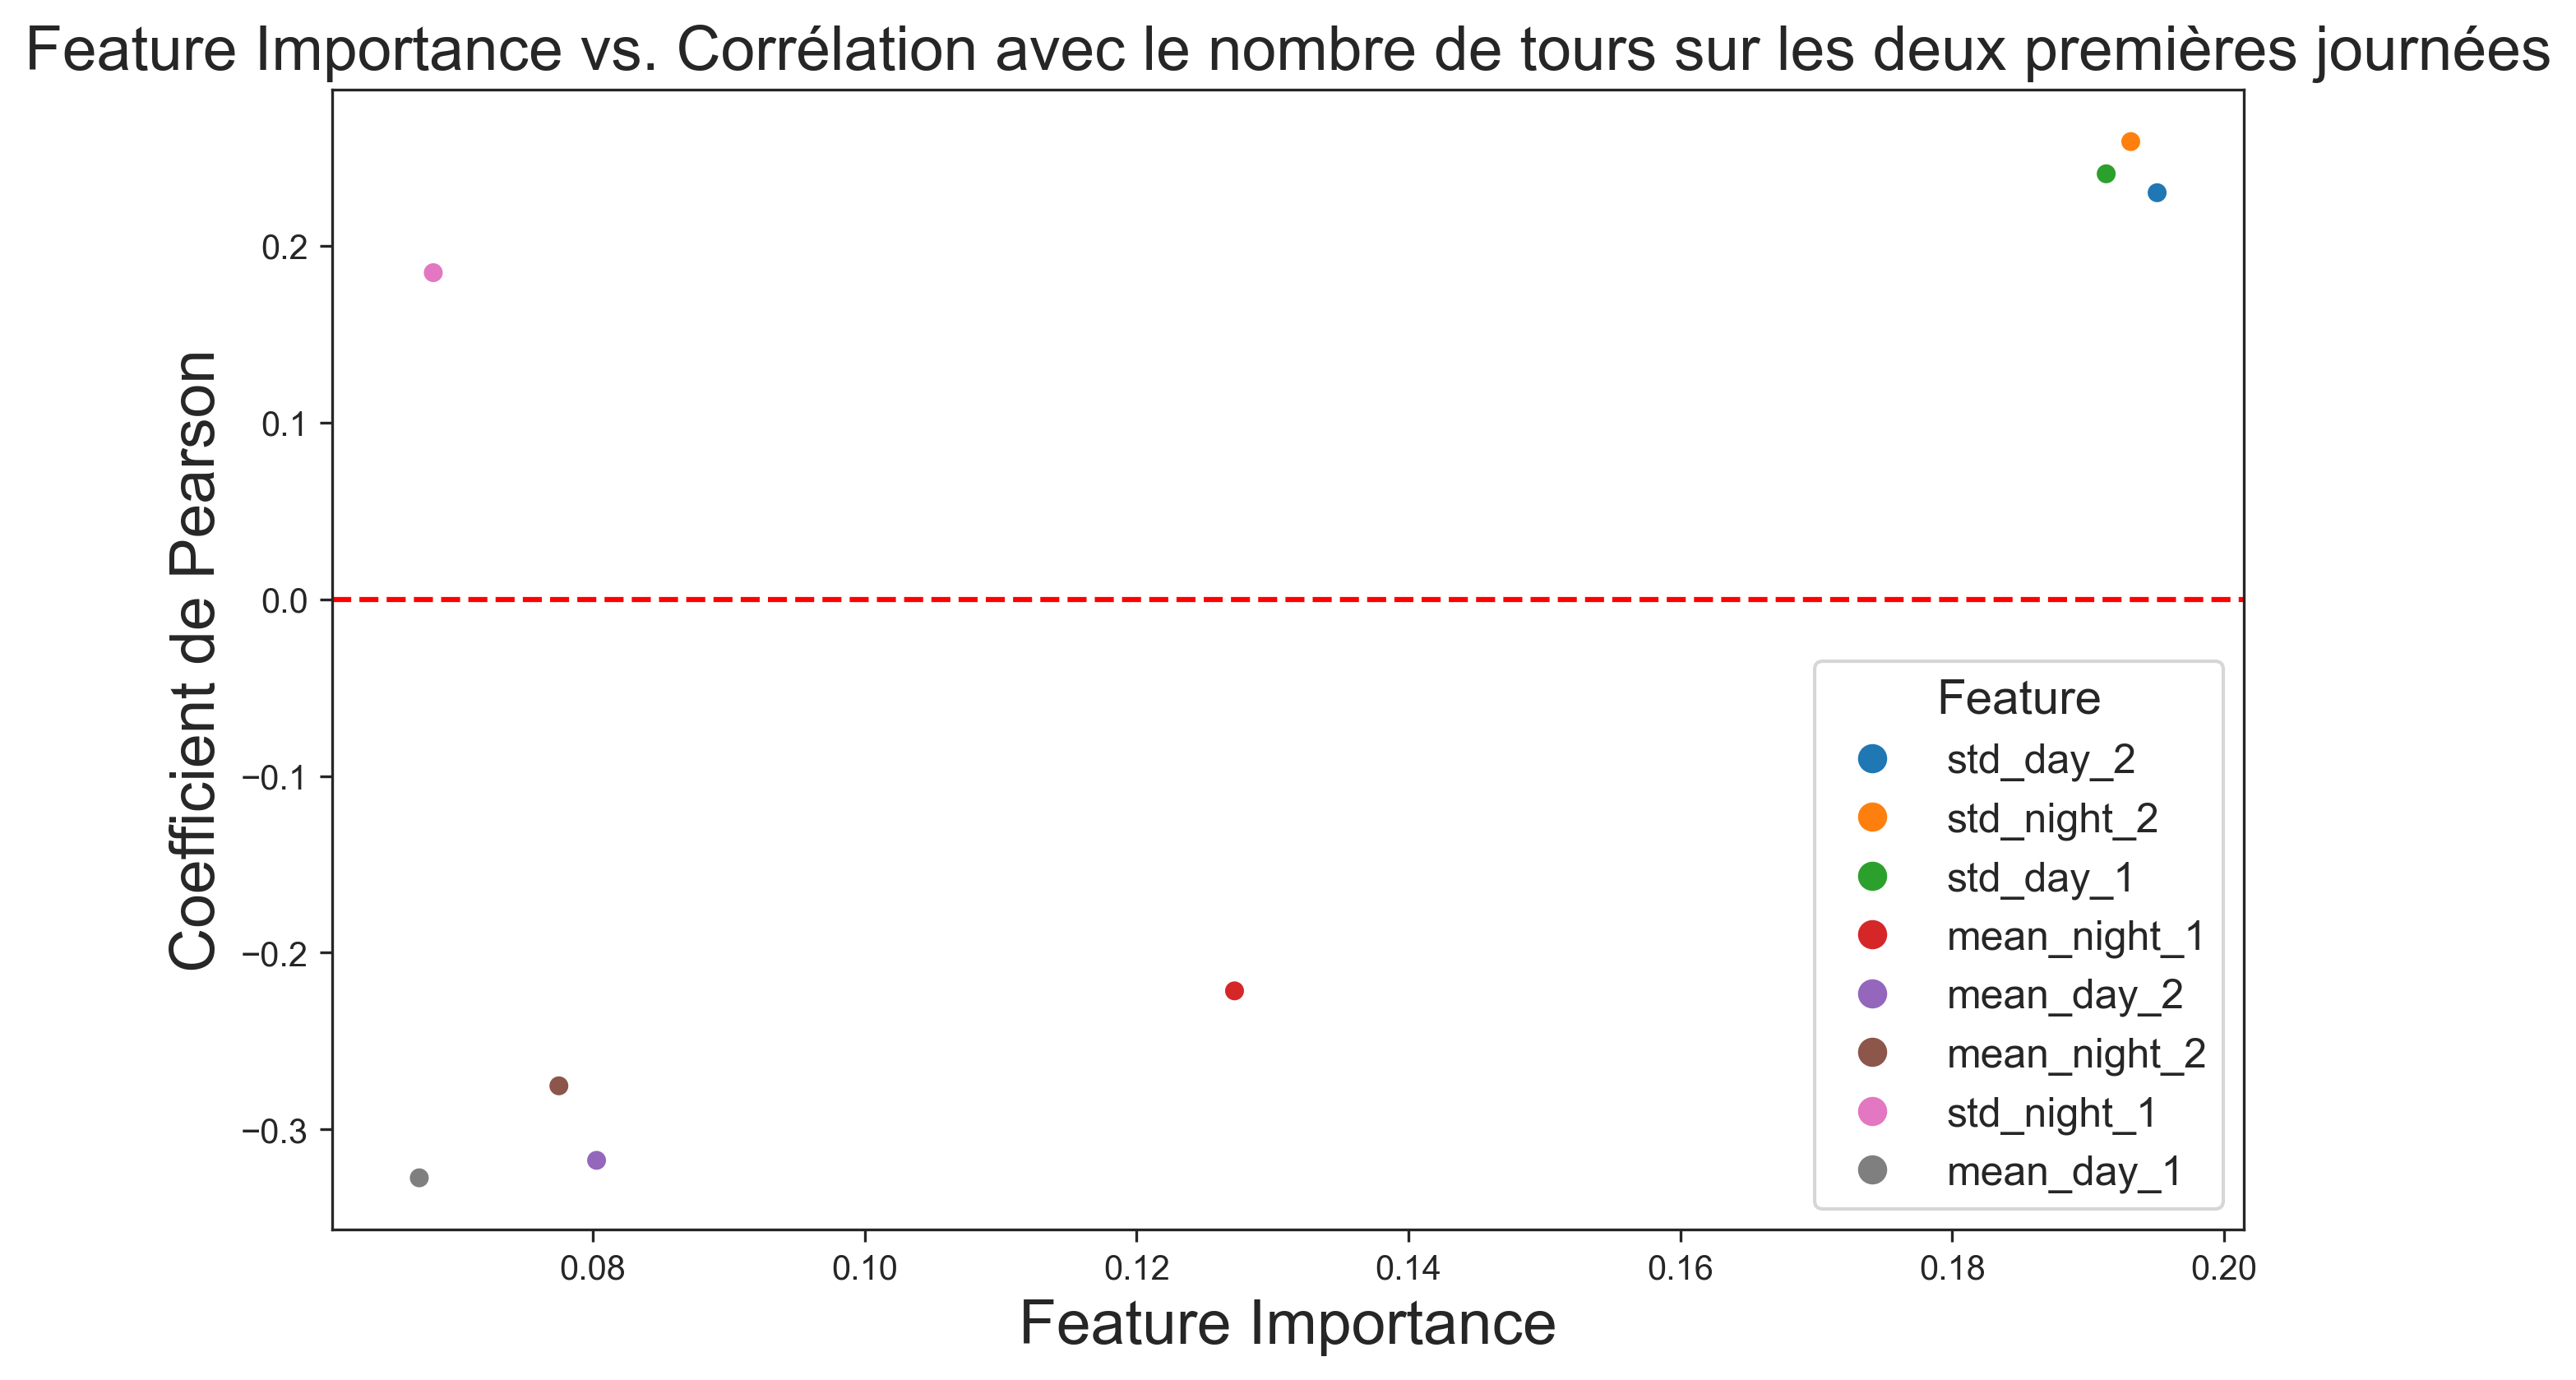
\includegraphics[scale=0.41	]{feature2}
	\centering
	\caption{Feature importance et corrélation sur les deux premiers tours}
\end{figure}

\medskip

Les résultats sont plutôt surprenants ! Ce qui semble le plus important pour effectuer un nombre élevé de tours est d'être irrégulier. N'oublions pas que cette analyse concerne uniquement les coureurs qui ont effectué 48 tours ou plus. 

\medskip

On peut effectuer la même analyse pour les coureurs ayant effectué 72 tours ou plus. C'est la variable \texttt{mean\_night\_3} qui est la plus importante, avec une corrélation négative. L'idée que les coureurs sur le point d'abandonner sont en souffrance reste valable. Ensuite, on retrouve la corrélation positive entre l'irrégularité et le nombre de tours. Essayons de trouver une explication. 

\begin{center}
	\textbf{Décryptage}
\end{center}
L'analyse de la feature importance des coureurs ayant effectué plus de 24 tours nous a appris qu'il fallait être assez rapide la première nuit mais aussi être régulier le premier jour. C'est l'idée intuitive que l'on a en prenant le départ de cette course: partir sur un rythme \textbf{régulier} que l'on peut maintenir longtemps. Les coureurs les plus forts sont ceux qui pourront maintenir ce rythme, les plus faibles auront plus de mal et seront donc plus lents la première nuit.

\medskip

En revanche, notre seconde analyse, qui porte sur les coureurs ayant effectué plus de 48 tours, nous donne une information qui contredit l'idée intuitive de la stratégie à adopter: il semble que les coureurs irréguliers ont plus de chance d'aller loin. Voici l'explication que je propose: Un coureur qui est régulier et qui part lentement pourra maintenir ce rythme 24, 48, peut être 72 heures, mais après la fatigue et le manque de sommeil se font de plus en plus ressentir. Un coureur plus irrégulier aura des tours plus rapides qui lui permettront d'avoir ponctuellement des moments de repos plus importants pour mieux s'alimenter, se changer et effectuer des micro-siestes. Lorsque la course s'étale sur quatre, cinq jours, ce sont les minutes de sommeil accumulés qui font la différence.

\medskip

Le bilan que l'on peut tirer de cette analyse est le suivant:
\begin{itemize}
	\item[$\bullet$] Si un coureur veut réaliser une bonne performance, il faut qu'il maintienne un rythme lent qu'il est capable de tenir longtemps et qu'il soit régulier. 
	\item[$\bullet$] Si un coureur veut jouer la victoire, il doit prendre des risques. Pour cela, il faut qu'il maintienne une allure modérée comme expliqué lors du point précédent mais ponctuellement, il doit effectuer des tours plus rapides afin d'avoir des moments de repos plus longs qui lui permettront de se ravitailler plus longtemps et surtout d'engranger des minutes de sommeil qui feront la différence lors des quatrième et cinquième jours.
\end{itemize}

\begin{center}
	\textbf{Recommandations pratiques sur la stratégie de course}
\end{center}

Après l'analyse de ces données, voici le plan de pacing que je proposerais.
\begin{itemize}
	\item[$\bullet$] Jour 1: Tours réguliers autour de 50 minutes avec 2 tours plus rapides (45 minutes) pour avoir des pauses plus longues pour bien s'alimenter, se changer... Compenser les tours rapides par des tours plus lents (53-54 minutes)
	\item[$\bullet$]Nuit 1: Tours réguliers autour de 45 minutes avec 3 tours plus rapides (38-40 minutes) pour s'accorder plusieurs micro-siestes. C'est assez risqué mais pour jouer la victoire, ce sont les minutes de sommeil accumulées qui feront la différence. Compenser avec des tours plus lents (47-49) minutes.
	\item[$\bullet$]Jour 2: Tours autour de 52 minutes. Même stratégie avec deux tours plus rapides (47 minutes) pour les mêmes raisons.
\item[$\bullet$]	Nuit 2: Tours autour de 48 minutes avec 3 tours rapides à 42-43 minutes pour les mêmes raisons.
	\item[$\bullet$]Jours suivants: la fatigue limite les temps au tour aux alentours de 54-55 minutes. Incorporer un tour plus rapide (50 minutes) si possible pour une bonne alimentation.
	\item[$\bullet$]Nuits suivantes: la fatigue limite les temps au tour aux alentours de 50 minutes. Incorporer un ou deux tours plus rapides (45 minutes) pour le sommeil si possible.
\end{itemize}

\medskip

Rendez-vous en 2025 pour analyser les performances des prochains championnats du monde solo !



	\end{document}